\section*{Ejercicio 2}

\subsection*{Analizar la siguiente red hallando la ecuación diferencia sin emplear Transformada Z:}

\begin{figure}[H]
    \centering 
    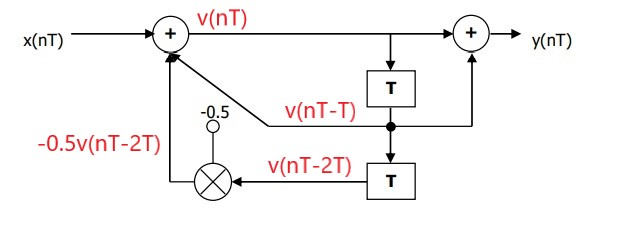
\includegraphics [scale=0.8]{images/ej2.png} 
    \caption{Diagrama}
\end{figure}

Sea v(nT) la señal a la salida de la adición, tal como se indica en el diagrama, luego por inspección se obtiene que:

$$y(nT) = v(nT) + v(nT-T)$$

Donde:

$$v(nT) = x(nT) + v(nT-T) - \frac{1}{2}v(nT-2T)$$

$$\therefore y(nT) = x(nT) + 2v(T(n-1)) - \frac{1}{2}v(T(n-2))$$